\chapter{Mobile robots}
\vspace{-0.5cm}
\minitoc

\begin{figure}[h]
    \centering
    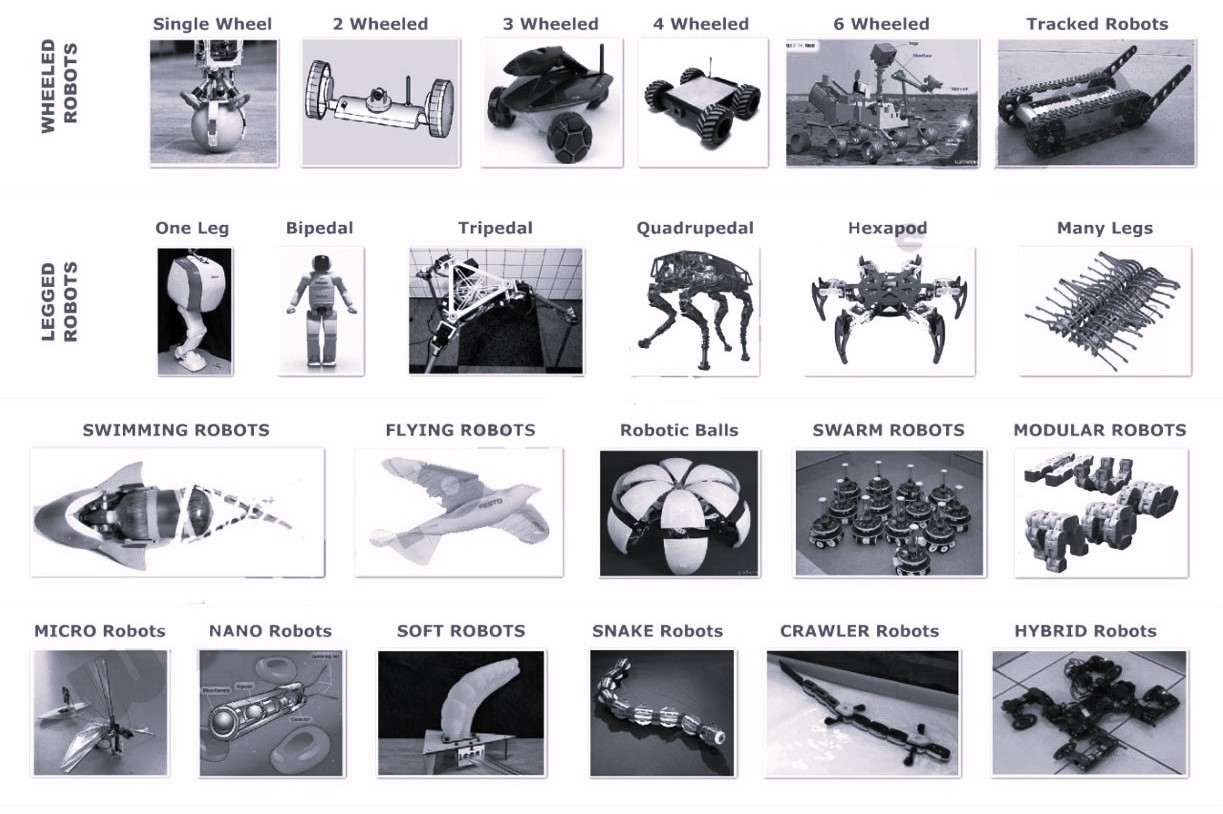
\includegraphics[scale=0.4]{img/classification.jpg}
\end{figure}
\vspace{-0.5cm}
\section{Introduction}
\begin{definition}[\textbf{Mobile robot}]
A \textbf{mobile robot} is a structure capable of moving and act in \textit{terrestrial}, \textit{underwater} or \textit{aerial} environments.    
\end{definition}
\noindent
The characteristics of the environment are fundamental since planning and control are affected by it. Namely the environment can be \underline{totally structured}, \underline{unstructured} or \underline{partially structured}. We refer the \textbf{structuredness} of the environment as the knowledge on geometric characteristics.
\subsection{Autonomy}
A mobile robot is equipped with a certain level of \textbf{autonomy} which makes the structure capable of moving independently from a human supervisor. For achieving it, it is required a computational part (CPU, Intelligence of the robot), some sensors and actuators and an energy source, which can be either generated on-board or provided by mean of an external source.
\subsection{Locomotion}
Another fundamental aspect is that, differently from manipulators, a mobile robot is equipped with a \textbf{locomotion apparatus} which drastically changes according to the environment they are acting in. A \textbf{terrestrial robot} can have wheels, legs or a biomimetic locomotion system; a \textbf{underwater robot} can provided with propellers or water jets; finally, an \textbf{aerial robots} can have rotating, fixed or flapping wings.

\section{Types of wheels}
In the following we are focusing our attention on the wheeled robots, as they represent the great majority of mobile robots used in applications. The basic mechanical structure of this robot is indeed the wheel. The table \Cref{tab:wheels} shows a summary of the fundamental information about the most popular types of wheels.

\begin{table}
    \centering
    \begin{tabular}{m{5cm} m{9cm} m{2cm} }
        \textbf{WHEEL TYPE}&\textbf{DESCRIPTION}&\textbf{SYMBOL} \\
        \toprule
        {\textsc{Simple non-steering wheel}}&{They can rotate about an axis which passes  through the center of the wheel itself, orthogonal to its plane. The orientation of the chassis with respect to the wheels is constant.}&{\centering 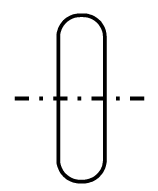
\includegraphics[scale=0.5]{img/simple_non_steering.png}} \\
        \midrule
        {\textsc{Simple steering wheels}}&{Has two axes of rotation, one that is orthogonal to the wheel plane, the other which is \textit{vertical} and goes through the center of the wheel. This provides the wheel with the possibility of changing the orientation with respect to the chassis. Note that for both non-steering and simple steering wheels the component the velocity which orthogonal to the wheel plane is null since there is no sleeping. That is: 
        \begin{equation*}
            v^{\perp}(t)=0
        \end{equation*}}&{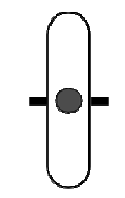
\includegraphics[scale=0.5]{img/simple_steering.png}} \\
        \midrule
        {\textsc{Castor wheel}}&{It is a variant of the previous one in which the vertical axis does not pass through the center of the wheel from which it is \textbf{displaced} by a constant offset. This adds degrees of freedom to the vehicle on which they are mounted on. Such a type of wheels are often used for office chairs and supermarket carts.}&{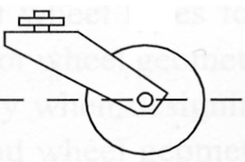
\includegraphics[scale=0.5]{img/castor_wheel.png}} \\
        \midrule
        {\textsc{Omnidirectional or Swedish wheel}}&{There is another type of non-conventional wheel that is the \textit{mechanum} (or \textbf{swedish wheel}). It mounts some passive rollers whose rotation axis is inclined by 45 degrees with respect to the plane of the wheel itself. They are also called \textit{omniwheels}.}&
        {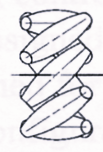
\includegraphics[scale=0.8]{img/swedish_wheel.png}} \\
        \midrule
        {\textsc{Spherical omniwheel}}&{There is another type of omniwheel which is \textbf{spherical}. They can be either active or passive. Like in the case of swedish wheels, a vehicle equipped with four of them is called \textbf{omnidirectional}.}& 
        {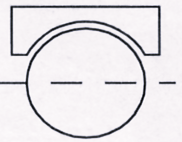
\includegraphics[scale=0.6]{img/spherical_wheel.png}}\\
    \end{tabular}
    \caption{Types of wheels with description and symbols}
    \label{tab:wheels}
\end{table}


\section{Constraints and Kinematic Models}
We have seen in the introduction that mobile and industrial robots have different characteristics, this results in different models, planning and control strategies. Since in general robots are made up of multiple rigid bodies (\textit{multibody system}) linked together by joints, their motion is constrained. This holds in general, however also the types of constraints are different in the case of mobile robots and manipulators. This is because in the former case you have limitations in the \textbf{position} of the whole body, in the case of mobile robots, and in particular in terrestrial wheeled robots, you have instead limitations on \textbf{how the position can change} in magnitude, direction and side (this is nothing but the \textbf{velocity}). From now on we are focusing our attention on \textbf{modeling wheeled robots}.

\subsection{Constraints and their classification}
In order to properly describing and giving a classification of constraints, it is better recalling the concept of \textbf{generalized coordinates}. \\
Let the vector $\mathbf{q}\in\mathbb{R}^n$ be the \emph{generalized coordinates} that describes the \textbf{configuration} of the robot (minimum number of variables needed to model the robot motion). For the moment, let us assume that the \textbf{configuration space} $\mathcal{C}$ coincides with $\mathbb{R}^n$. For example for a \textbf{unicycle} the generalized coordinates are in number of three: 
\begin{equation}\label{eq:gen_coord_unicyle}
    \mathbf{q}=[x \quad y \quad \theta]^T\in\mathbb{R}^3
\end{equation}
where $x$ and $y$ are the position of the contact point between the (single) wheel and the plane on which the motion occurs, while $\theta$ is the angle of the wheel with respect to the horizontal axis. The \textbf{evolution in time} of the generalized coordinates vector \textit{describe the motion} of the system.\\

Constraints can be found by mean of \textbf{equality} (in this case we refer them as \textit{bilateral} constraints), by mean of \textbf{inequality} (we refer them as \textit{unilateral} constraints). Furthermore, according to the fact they are or not time-variant, we can divide them in \textit{rehonomic} (explicit dependence on time) and \textit{scleronomic} (time-invariant constraints). In this course we will treat only \textbf{bilateral and scleronomic constraints} another term for indicating them is \textbf{holonomic} (or \textbf{integrable}) constraints.

\subsubsection{Holonomic constraints}
Such a type of constraint\footnote{
    We recall that for a multibody system described by using the Lagrangian approach, holonomic constraints are those allowing a reduction of the number of needed variables.
} can be expressed as: 

\begin{equation}
    h_i(\mathbf{q})=0, \quad i=1,...,k<n
\end{equation}

A system whose motion is characterized only by holonomic constraints is called \textbf{holonomic system}. By using the \textit{implicit function theorem} (or in Italian "Teorema del Dini"), we can reduce the dimension of the configuration space to $n-k$

\subsubsection{Kinematic constraints}
Such a type of constraints involve both generalized coordinates $\mathbf{q}$ and its derivative $\dot{\mathbf{q}}$. In the most general case they can be expressed as:
\begin{equation}
    a_i(\mathbf{q},\dot{\mathbf{q}})=0, \quad i=1,...,k<n   
\end{equation}
Kinematic constraints are limiting the set of generalized velocities that can be obtained by each configuration. In some cases they can be written in the so-called \textbf{Pfaffian form}, that is they can be written as a \textit{linear combination of the generalized velocities $\dot{\mathbf{q}}$}: 
\begin{equation}
    \mathbf{a}_i^T(\mathbf{q})\dot{{\mathbf{q}}}=0, \quad
    i=1,...,k<n
\end{equation}
An example of kinematic constraint in Pfaffian form is:
\begin{equation*}
    3q_1 \dot{q}_1 +
    2 \sin{q_1}\dot{q_2}+
    \sin{q_3} \dot{q}_3 =0   
\end{equation*}
The reason for using such a notation is that we can immediately retrieve the expression of the associated function by doing the row-by-column product (standard inner product). Such $k$ kinematic constraints can be written in compact form by introducing matrices
\begin{equation}\label{eq:matrix_pfaffian}
    \mathbf{A}^T(\mathbf{q})\dot{\mathbf{q}}=\mathbf{0}
\end{equation}
where $\mathbf{A(q)}\in\mathbb{R}^{k,n}.$ It is interesting to note that the presece of $k$ holonomic constraints imply the presence of $k$ kinematic constraints. This can be easily showed by computing the time derivative for the $k$ holonomic constraints: 
\begin{equation}\label{eq:kin_holonomic}
    \frac{d h_i(\mathbf{q})}{dt}=
    \frac{d h_i(\mathbf{q})}{d\mathbf{q}}\cdot
    \frac{d \mathbf{q}}{dt}=
    \frac{d h_i(\mathbf{q})}{d\mathbf{q}}\cdot \dot{\mathbf{q}}=0, \qquad
    i=1,...,k
\end{equation}
where we have applied the fact that the constraints are holonomic while using the \textit{Chain rule} for passing from the first to the second step. From the \Cref{eq:kin_holonomic} we have understood that: 
\begin{equation*}
    \text{holonomic constraint} \Longrightarrow 
    \text{kinematic constraints}
\end{equation*} 
In general, we cannot say the inverse and in this case (since the step from the derivative to the primitive results in doing the integral) associated constraints are called \textbf{nonholonomic} (or \textbf{non-integrable}) ones. A system characterized by such constraints is called \textbf{nonholonomic system}. In presence of non-integrable constraints the dimension of the configuration space $\mathcal{C}$ cannot be reduced while the generalized velocities can be described over a subspace of dimension $n-k$ (how we are going to see in a minute).

\subsubsection{Example of nonholonomic constraint}
A unicycle rolls on a plane \textbf{without slippering}, we have already seen its generalized coordinates. For such a system we have the so called \textbf{pure rolling constraint}, this imply the velocity of the contact point not to have a non-zero component along the direction orthogonal to the wheels plane. By using simple trigonometric properties involving the inifinitesimal increment $dx$ and $dy$, we can state that
\begin{equation}
    \frac{dy}{dx}=\tan{\theta}
\end{equation}
Can we obtain the Pfaffian form for such a constraint? The answer is YES. In fact by dividing and multiplying for an infinitesimal time increment $dt$ we obtain:
\begin{equation*}
    \frac{dy}{dx}=\frac{dy}{dt}\cdot
    \frac{dt}{dx}=\frac{\dot{y}}{\dot{x}}=\frac{\sin\theta}{\cos{\theta}} \iff 
    \dot{y}\cos{\theta}=\dot{x}\sin{\theta}
\end{equation*}
Which is the same to say that
\begin{equation}
    \dot{x}\sin\theta-\dot{y}\cos{\theta}=0 \iff 
    [\sin\theta \quad \cos\theta \quad 0] \dot{\mathbf{q}}=0
\end{equation}
The constraint we have just derived can be demonstrated that is non-integrable and so nonholonomic, in fact we cannot reduce the dimension of the configuration space (in other words all of the generalized coordinates are needed to properly describe the unicycle motion). Note that, start from an initial state $\mathbf{q}_i$, you can bring the system to any final state $\mathbf{q}_f$, under the assumption of not to violating the pure rolling constraint\footnote{
    We will see that in order to pass from an initial to a final state a \textit{trajectory planning algorithm} must be used.
}.

\subsection{Kinematic model}
From the \Cref{eq:matrix_pfaffian}, we can immediately see that the $n-k$ admissible generalized velocities belong to the null space\footnote{
    Just for doing a brief recap. Given a matrix $A\in\mathbb{R}^{m,n}$ we can individuate the following sets (vector spaces):
    \begin{itemize}
        \itemsep-0.3em
        \item \textsf{Null space} that is the a subset of $\mathbb{R}^n$ defined as: 
        \begin{equation}
            \mathcal{N}(A)=\{x\in\mathbb{R}^n: \ Ax=0\}
        \end{equation}
        \item \textsf{Range space} that is a subset of $\mathbb{R}^m$ defined as: 
        \begin{equation}
            \mathcal{R}(A)=\{y\in\mathbb{R}^m: \ y=Ax\}
        \end{equation}
        the dimension of such a vector space is called the rank of the matrix A (rank(A)) and it holds that its maximum value is the $\min(m,n)$.
    \end{itemize}
    Another important result is that
    \begin{equation*}
        n=\dim{\mathcal{N}(A)}+\dim{\mathcal{R}}(A)
    \end{equation*}
    Knowing $n$ (for us dimension of the configuration space)
 and the rank of A, we can find the dimension for the null space of A.} of $\mathbf{A(q)}^T$ that is 
\begin{equation}
    \dot{\mathbf{q}} \in \mathcal{N}(\mathbf{A^T(q)})
\end{equation}
We know that this is a vector space and it has got a basis of $n-k$ elements which we can denote with $\{\mathbf{g}_i(\mathbf{q})\}_{i=1}^{n-k}$, we can group together such elements in a matrix $\mathbf{G(q)}$ so that the generalized velocities can be expressed as
\begin{equation}
    \mathbf{\dot{q}=G(q)u}
\end{equation}
this is nothing but the \textbf{kinematic model} of the constrained system (a system of ordinary differential equations\footnote{ODE}). The vector $\mathbf{q}$ is called the \emph{state vector} while $\mathbf{u}$ is the \textbf{input vector}. Moreover the obtained system is said to be driftless since in absence of an input the generalized velocity is null. Not rarely the components $u_i$ of \textbf{u} have a meaning related to the physics or the available control input.\\

In the following for better fixing the concepts we have just given, two example of kinematic models are given.

\subsubsection{Kinematic model for the unicycle}
Let us consider, a bit more in details, the unicycle system. It is noticeable that the line in which the motion does not occur is called \textbf{zero motion line}.\\
We have said that the generalized coordinated $\mathbf{q}$ are the ones in \Cref{eq:gen_coord_unicyle}. We have a single constraint that we have reduced in Pfaffian form. The next step \emph{in order to obtain a kinematic model} is determining a base for the null space of the constraint matrix. One possible choice for vector fields $\mathbf{g_i(q)}$ is\footnote{
    Note that this is a vector field since both domain and codomain are vectors of suitable dimensions.
}:
\begin{equation*}
    \mathbf{g}_1(\mathbf{q})=\begin{bmatrix}
        \cos\theta&\sin\theta&0
    \end{bmatrix}^T, \quad
    \mathbf{g}_2(\mathbf{q})=\begin{bmatrix}
        0&0&1
    \end{bmatrix}^T
\end{equation*}
\begin{multicols}{2}
    \noindent
    Therefore, putting them together we obtain the matrix
\begin{equation}
    \mathbf{G(q)}=\begin{bmatrix}
        \cos\theta&0\\
        \sin\theta&0\\
        0&1
    \end{bmatrix}
\end{equation}
The kinematic model for the unicyle, then, can be written as:
\begin{equation}
    \begin{bmatrix}
        \dot{x}\\\dot{y}\\\dot{\theta}
    \end{bmatrix}=\begin{bmatrix}
        \cos\theta\\
        \sin\theta\\
        0
    \end{bmatrix}v+\begin{bmatrix}
        0\\0\\1
    \end{bmatrix}\omega
\end{equation}
\\
\begin{figure}[H]
    \centering
    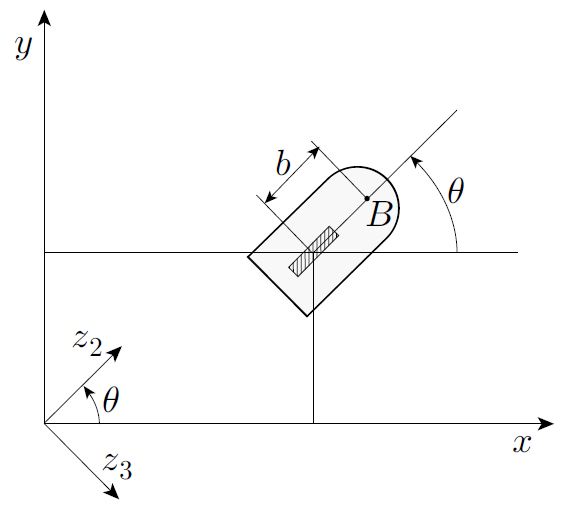
\includegraphics[scale=0.6]{img/unicycle_scheme.png}
    \caption{Choice of generalized coordinates for the unicycle}
    \label{fig:unicycle_model}
\end{figure}
\end{multicols}
In such a context the elements of the input vector have a physical meaning, since $v$ is the driving velocity, while $\omega$ is nothing but the steering velocity.  Why are we interested in studying the kinematic model of a unicyle? Consider that without a human beings balancing the system this is also an unstable system! However, there are some robot (stable) robot structures that from a \textbf{kinematic point of view} are equivalent to unicycles. We are talking about \emph{differential drive} and \emph{synchro drive} vehicles.

\subsubsection{Differential drives: a stable structure for the unicycle model}
A \textit{differentially driven robot} has two independent wheels with different angular velocities $\omega_R$ and $\omega_L$. Both wheels have a radius $r$ and are constrained to be at a distance $d$. A third wheel is passive, in the sense that there is not a motor changing that velocity. By doing a proper choice for the control input, we can obtain a kinematic model that is totally equivalent to the one of a unicycle. In particular, from the left and right wheels angular velocities we can obtain: 
\begin{align}
    &v=\frac{r}{2}{(\omega_R+\omega_L)}\\
    &\omega=\frac{r}{d}{(\omega_R-\omega_L)}
\end{align}

\subsubsection{Kinematic model for a bicycle}
A \textbf{bicycle} is vehicle with a steered wheel and a fixed one, the distance between the wheels is fixed to be $L$. As usual we have to choose the (generalized) coordinates for such a vehicle a possible choice is the following:
\begin{itemize}
    \itemsep-0.3em
    \item $(x,y)$ being the contact point of the rear\footnote{
        back wheel
    }; 
    \item $\theta$ is the angle between the rear wheel and the $x$ axis (this is nothing but the orientation of the vehicle with respect to the $x$ axis); 
    \item $\phi$ is the steering angle of the front wheel.
\end{itemize}
\begin{remark}
    It is interesting focus our attention on a point: why do not we introduce also the coordinates of the front wheel? Well, it is sufficient having a single contact point since, back and front wheel are at a fixed distance $\ell$, and this is nothing but an \textit{holonomic constraint} which allows us the shrinking of the configuration space dimension! 
\end{remark}
Going on into the discussion, there are essentially two \textit{pure rolling constraints}, one for each wheel: 
\begin{align}
    &\dot{x}_f \sin(\theta+\phi)-\dot{y}_f \cos(\theta+\phi)=0 \label{eq:front_pure_rolling}\\
    &\dot{x}\sin(\theta)-\dot{y}\cos(\theta)=0
\end{align}
while indicating with $(x_f,y_f)$ the coordinates of the front wheel center, while $(\theta+\phi)$ is its angle with respect to the fixed reference frame. We have just said that they are not strictly necessary, since they can be obtained starting from the coordinates of the other wheel in particular: 
\begin{equation}
    \begin{cases}
        x_f=x+\ell\cos\theta\\
        y_f=y+\ell\sin\theta
    \end{cases}
\end{equation} 
using the trigonometry, the \Cref{eq:front_pure_rolling} can be expressed as
\begin{equation}
    \dot{x}\sin(\theta+\phi)-\dot{y}\cos(\theta+\phi)-\ell\dot{\theta}\cos(\phi)=0
\end{equation}
where we have used that $\sin^2\theta+\cos^2\theta=1$ and the trigonometric formulas for $\cos(\theta+\phi)$ and $\sin(\theta+\phi)$. The derived constraints can be put if Pfaffian form using the matrix
\begin{equation}
    \mathbf{A}^T(\mathbf{q})=\begin{bmatrix}
        \sin\theta&-\cos\theta&0&0\\
        \sin(\theta+\phi)&-cos(\theta+\phi)&-\ell\cos\phi&0
    \end{bmatrix}
\end{equation}
\newpage
\begin{multicols}{2}

Our objective is obtaining a basis for the null space of such a matrix in order to derive the kinematic model. Since $rank(\mathbf{A^T(q)})=2$, the dimension of its null space is given by the difference between the dimension of the configuration space and such a rank, that is 2. A possible basis for such a null space is given by the column of
\begin{equation}
    \mathbf{G(q)}=\begin{bmatrix}
        \cos\theta\cos\phi&0\\
        \sin\theta\cos\phi&0\\
        \frac{\sin\theta}{\ell}&0\\
        0&1
    \end{bmatrix}
\end{equation}
\begin{figure}[H]
    \centering
    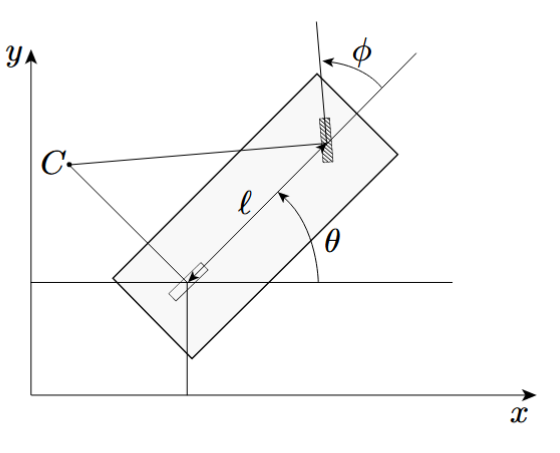
\includegraphics[scale=0.6]{img/bicycle_scheme.png}
    \caption{Possible choice for the generalized coordinates of a unicycle}    
    \label{fig:scheme_bicycle}
\end{figure}
\end{multicols}
\noindent
The associated kinematic model is:
\begin{equation}
    \begin{bmatrix}
        \dot{x}\\
        \dot{y}\\
        \dot{\theta}\\
        \dot{\phi}
    \end{bmatrix}=\begin{bmatrix}
        \cos\theta\cos\phi\\
        \sin\theta\cos\phi\\
        \frac{\sin\theta}{\ell}\\
        0
    \end{bmatrix}u_1 + \begin{bmatrix}
        0\\
        0\\
        0\\1
    \end{bmatrix}\omega
\end{equation}
the control input $u_1$ can be choosen according to the drive in particular $u_1=v$ if the vehicle is front-drive, $u_1=v/\cos\theta$ if the vehicle is back drive, since the first two equations must be equivalent to the ones of a unicyle. Just for a matter of notation/nomenclature the instersection point $C$ between the two zero motion lines is called \textit{instantaneous center of rotation}, depends only on $\mathbf{q}$ and it is interesting since each point of the chassis is moving instantaneously along along the circumference centered at $C$ (see \Cref{fig:scheme_bicycle}).\\
Equivalent (stable) systems having the same kinematic model are the \textbf{tricyle} and the \textbf{automobile}.\\
An interesting point is that, if we assume that the steering velocity can be \textit{manually controlled}, the number of state variables (generalized coordinates) for the bicycle is the same than the unicycle. In this way we can model both systems using the same kinematic model.
\begin{remark}
    We remind that the kinematic model represent a system of ODE which can be solved using any integration method available in MATLAB. For example we can obtain the trajectory of the unicycle/bicyle model and the time law for $\theta$ by using the command \texttt{ode45}.
\end{remark}

\section{Sensors for mobile robots}
Sensors play a crucial role in the field of robotics and mobile robots. They are, approximately, devices which takes measurement from the environment and convert them in a form which can be further analyzed by the computer of which the robot is equipped.\\
Before focusing on sensors, let us give the definition of what a \textbf{transducer} is. This is a device by a ehich signal from one form of energy (eg. mechanical) is converted into another form of energy. Moreover can be either \textit{emitters} or \textit{receivers}.\\
\textbf{Sensors} are receivers which covert a measurable signal intol an electric one. Very often in order to be digitally elaborated, such signals are converted by using an ADC device.\\

In the following, after giving some possible classifications and features about sensors, we introduce the main types of such devices used in the field of robotics and in particular in the field of \textit{mobile robotics}.

\subsection{Sensors classification and features}
There are different classifications can be done about sensors, each one focusing on a different aspect:
\begin{itemize}
    \itemsep-0.3em
    \item \textsf{Passive/Active sensors} the former ones measure the energy from the environment directly the latter ones at first inject some form of energy (eg. light) and then they measure the effects such energy produces.
    \item \textsf{Proprioceptive/Exteroceptive sensors} is a classification based on what type of measurements the sensors themselves are taking. A \textit{proprioceptive} sensor takes measures of quantities related to the robot (internal), the other are taking the measurement with reference to the \textit{external world}.
    \item \textsf{Type of taken measurement} in the sense that there are sensors measuring contact, position, velocity and so on.
\end{itemize}
In the \Cref{tab:sensfeature} we are going to give main characteristics and features for common sensors.

\begin{table}
    \centering
    \small
    \begin{tabular}{p{5.5cm} p{9.5cm}}
        \toprule
        \textbf{FEATURE}&{\textbf{DESCRIPTION}}\\
        \midrule\midrule
        \textbf{Linearity and nonlinearity}&{A sensor if the relationship between its input and the related output is linear. Such sensors result (approximately) in simple models, moreover the \textit{effect of noise} is also linear in the sensor range.
        }\\
        \midrule
        \textbf{Measurement range}&{A sensor cannot take whatever measurement. In particular, they are in a certain interval with a smallest and a largest value. Namely $Range=[A,B]$}\\
        \midrule
        \textbf{Dynamic range}&{It is nothing but the ratio between $B$ and $A$ expressed in dB, that is:
        \begin{equation*}
            \text{Dynamic range}=20\log_{10} \frac{B}{A}
        \end{equation*}}\\
        \midrule
        \textbf{Sensitivity}&{Is nothing but the slope $dy/dx$ of the sensor response. An accurate sensor should have \textit{high sensitivity}. If it is a linear one such a parameter (the derivative) is constant. The sensitivity can be used in order to detect the saturation: you have saturation when to input variation, there is no output variation. Such a phenomenona occurs outside the \textit{measurement range}}\\
        \midrule
        \textbf{Resolution}&{Is the minimum variation of the measured physical variables that can produce a detectaable change in the ouptut. It can be associate to either physical limitations or ADC process}\\
        \midrule
        \textbf{Precision}&{It represents the metric about the \textit{reproducibility} of given measurements. Ideally one would have the same measurement again and again, real sensors provide a \textit{range of values} over time which are distributed according to a certain statistical distribution.}\\
        \midrule
        \textbf{Accuracy}&{It is a metric quantifying the \textit{correctness} of the output provided by a sensor compared to the real value of the measured signal. The concept of \textit{real value} can turn in a philosophical one. For this reason, accuracy is assesses by taking in relation with other more accurate devices.}\\
        \midrule
        \textbf{Bandwidth}&{It is known as the \textit{maximum frequency} at which the sensor provides reliable measurements. We want the sensor bandwitdth to be sufficiently, but not too much, large so that the noise (tipycally high frequency signal) is avoided.}\\
        \midrule
        \textbf{Response time}&{Is the time which elapses between the change in the input and the associated variation of the sensor output. }\\
        \bottomrule
    \end{tabular}
    \caption{Sensors characteristics and features}
    \label{tab:sensfeature}
\end{table}

\subsection{Proximity and contact sensors}
They are used from mobile robots in order to sense object which are either in front of them or nearby, at a distance that is fixed or parametrizable. The most general family is known as \textit{proximity sensors}, when the distance is zero (within a certain tolerance), these are \textit{contact sensors}. Such a type of robot can be used for both safety or navigation tasks. The most common forms in which you can find them are:
\begin{enumerate}
    \itemsep-0.3em
    \item \textit{Photoelectric proximity} Uses a couple LED + Photoresistor in otder to sense the reflected light. It may receive a signal which is proportional to the distance.
    \item \textit{Bumpers} Such devices present as \textit{microswitches} attached to the protective case and they are used to receive shocks and then to sense the contact.
\end{enumerate}
One example for both types is shown in \Cref{fig:proximity}.

\begin{figure}
    \centering
    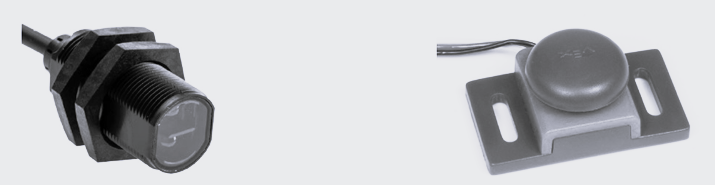
\includegraphics[scale=0.7]{img/sens_proximity.png}
    \caption{Proximity and contact sensors. From left: photoelectric and bumper}
    \label{fig:proximity}
\end{figure}

\subsection{Encoders}
This are part of the \textit{proprioceptive sensors} and are devices which converts a \textbf{linear or angular position} into a digital code. The building block of any type of encoder is a \textit{disc} subvided in sectors embedded with a mechanism to count sectors. They are substancially based on optical mechanism or exploit the Hall effect.

\begin{figure}
    \centering
    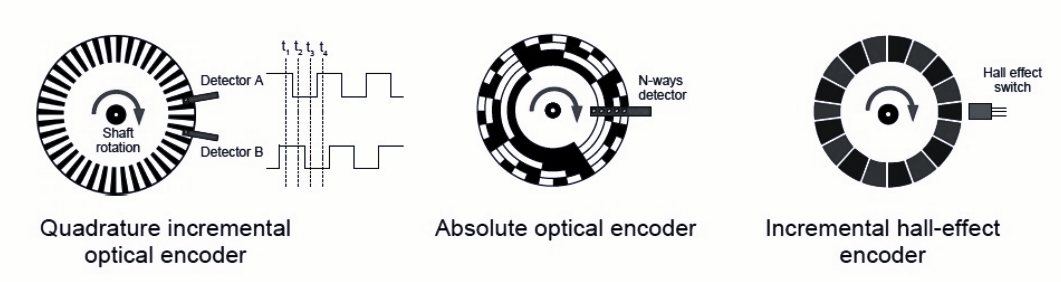
\includegraphics[scale=0.7]{img/sens_encoder.png}
    \caption{Different types of encoder}
\end{figure}

\subsection{Global Positioning Systems}
In the case of \textit{GPS (Global Positioning System)} the localization is made possible through a set of distinguished landmarks of beacons. Such a type of localization can occur either outdoor (in the nature) or indoor (in a closed place). Different protocols are used in both cases.

\subsubsection{Outdoor positioning: GNNS}
\textbf{GNSS} stands for \textit{Global Navigation Satellite System Receivers} here a receiver (put on the robot) can sense signals from a subset of \textbf{satellites}. Using the time of arrival of such a signal the \textit{distance can be estimated}. Using the trilateration, \textit{latitude, longitude} and \textit{elevation} can be found. This is the basic version of the protocol. However there are some variants: 
\begin{description}
    \itemsep-0.3em
    \item[DPGS] (Differential Global Positioning System) The GPS receiver communicates with one or more base stations (on the Earth)  in order to correct common error related to the transmission from the satellites to the Earth ground. Accuracy is of the order of meters.
    \item[RTK] (Real time kinematics) Here instead of analzying only the time of  arrival also the carrier wave is used. The distance is inferred from the number of cycles to which is added the phase difference. In particular, the  \textit{phase difference} is provided by a base station which serves a certain number of satellites. This technique provides a fine-grained correction of the measurement, in this way the accuracy passes from meters to centimeters.
\end{description}

\begin{figure}[h]
    \centering
    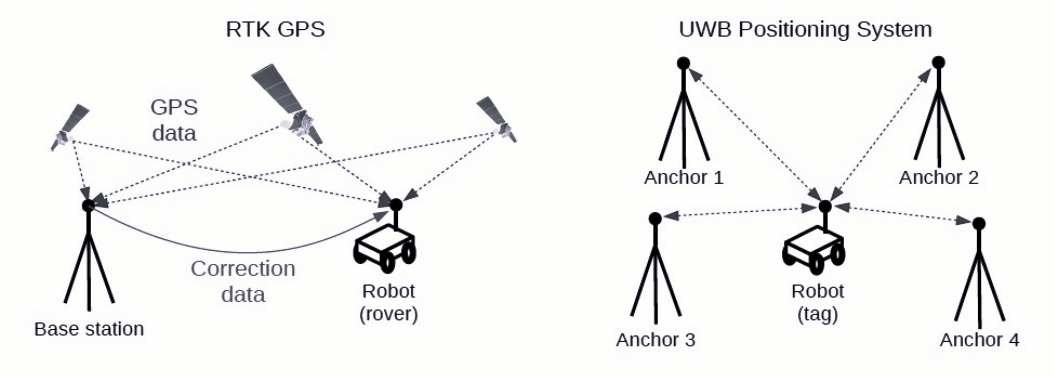
\includegraphics[scale=0.7]{img/sensor_GPS.png}
    \caption{Global Positioning System}
\end{figure}

\subsubsection{Indoor positioning: UWB}
\textbf{UWB} (Ultra-wideband positioning system) is based on the same concept of GNSS. However there are some differences: (i) some \textit{anchors} are used with a frequency in the range $[3.1,10.6]$GHz; (ii) The communicaiton is bidirectional and the 3D localization can be achieved by mean of a 3D placement of the anchors. Note that each robot being localized by using UWB must be equipped with a \textbf{UWB tag}. Even in this case different strategies are used.

\begin{description}
    \itemsep-0.3em
    \item[TDOA] (Time difference of arrival) In this case the UWB tag constantly broadcast a message with its own identity. The anchors will receive such a signal with \textit{time differences} since the position is different. If the anchors are all synchronized on the same clock signal, is possible performing the localization by using trilateration.
    \item[TOF] (Time of flight) This technique is applied when there is the absence of a \textit{global clock}. In particular, a 2-way protocol is used: a message is sent by using the UWB tag and a control message is bounced back. The distance from the anchors is obtained by computing the \textit{time of flight}, finally trilateration is applied to retrieve the indoor positioning.
\end{description}

%---------------------------------------------------------
\subsection{Inertial and Heading Sensors}
There are some sensors which use the \textbf{inertia}\footnote{
    It is the property of a body to change its current state of stillness of motion with constant linear or rotational velocities.
} of the body to retrieve position and orientation of the body itself. Such sensors are mainly \textbf{accelerometers} and \textbf{gyroscopes}.

\subsubsection{Accelerometers}
Their objective is to measure the \textit{linear acceleration} along a defined axis, such an acceleration is typically converted into either a force or a deformation (mass-spring based). There are both \textit{piezoelectric} and \textit{capacitive} sensors.

\begin{figure}
    \centering
    \subfigure[Accelerometer]{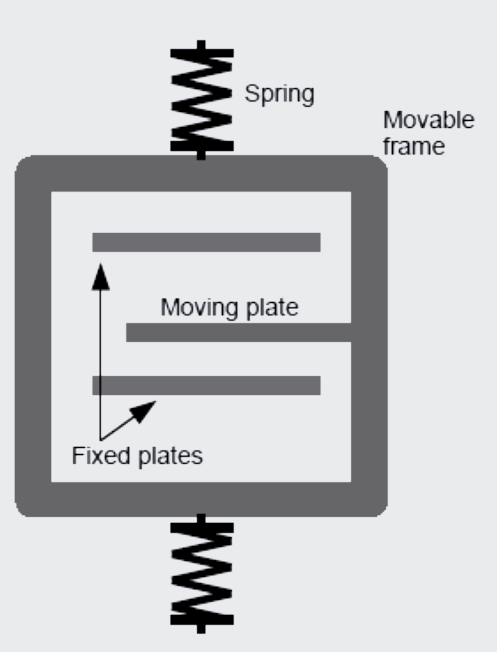
\includegraphics[scale=0.5]{img/sens_accelerometer.png}}
    \subfigure[Gyroscope]{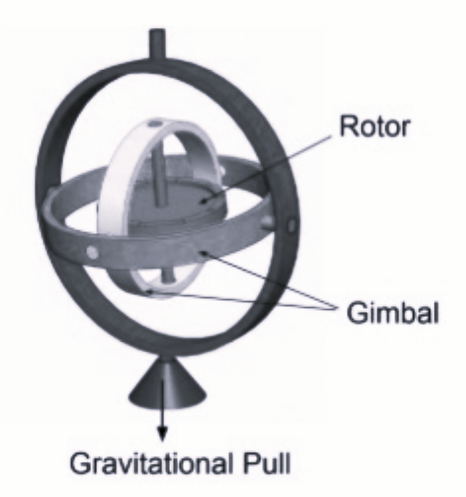
\includegraphics[scale=0.6]{img/sens_gyroscope.png}}
    \subfigure[IMU]{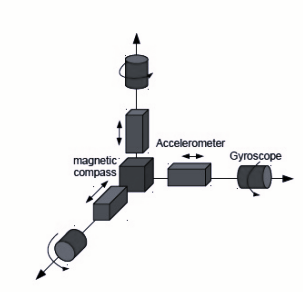
\includegraphics[scale=0.7]{img/sens_IMU.png}}
    \caption{Inertia and Heading sensors}
\end{figure}

\subsubsection{Gyroscopes}
They are used for measuring the orientation of a body using a vibrating or rotating body which tends to preserve the initial body's orientation. They can assume the following forms: 
\begin{description}
    \itemsep-0.3em
    \item[Rotating Structure Gyroscopes] They use a disk which is mounted on a structure which allows the orientation of the body to be unchanged when the whole structure itself is rotated. The orientation is obtained by computing the differences between the starting and final relative position of the body with respect to the rest of the gyroscope. Non-idealities due to friction must be taken into account for more accurate results.
    \item[Vibrating Structure Gyroscopes] They exploit the \textit{vibration of a body} along the same direction irrespective with the rotation of the sensor itself. The vibration produces a force, whose measurement is able to provide the \textbf{rate of rotation}. The absolute orientation is obtained by mean of integration.
\end{description}

\subsubsection{Compasses}
They are used in order to measure the direction of the Earth's magnetic field (N-S). This can be made using the \textit{Hall effect} or the \textit{Fluxgate} principle. In the former case is exploited the phenomena according which when a conductor is traversed by a current. In presence of a magnetic field a voltage is generated in the orthogonal direction of the current. In the latter case a measurement of a \textit{magnetic flux} is exploited.

\subsubsection{Inertia Measurement Units (IMUs)}
An IMU is a device which embeds in a single device all of the Inertia sensors we have seen till now. In particular there is a compass and three couples (Accelerometer, Gyroscope) along the three axis of motion. They are often used to improve the performance of the GPS.

%---------------------------------------------------------
\subsection{Digital cameras}
They are particular devices which produces 2D arrays, by mean of an image, containing the measurement of the \textit{visible light} from a 3D scene. You can imagine that, since a 3D scene is transformed into a 2D array, the third dimension is lost. Main components of cameras are: (i) a imaging sensor, (ii) lens to route the light toward the sensor, (iii) an ADC to convert each pixel into a digital value. Ideally, we wish to reproduce the \textit{pinhole model} in which each single 3D point is mapped into a single pixel realizing the so-called \textit{perspective transformation}. There are mainly two types of cameras: (i) \textit{gray level cameras} give as an output a brightness map which is a  measure of the intensity of the elctromagnetic radation; (ii) \textit{Color cameras} measure also the wavelength of such a radiation. In particular, they use separate sensors which are sensitive to different wavelenghts.


\subsubsection{Omnidirectional cameras}
Vanilla cameras provide a limited field of view. \textit{Omnidirectional cameras} solve this issue by achieving a field of view of 180° in both horizontal and vertical directions. \textsf{fisheye lens and mirrors} are used. The pinhole model does not hold anymore, the \textit{spherical projection model} is used instead.

\subsubsection{Event cameras}
Standard cameras provide data at a fixed rate (tipically 50-60 frame per second). \textit{Event cameras} are equipped with \underline{asynchronous sensors} that generates a series of timestampe events wheter the brightness of the image changes. They are used in task in which is important achieving a certain level of performance.

\begin{figure}
    \centering
    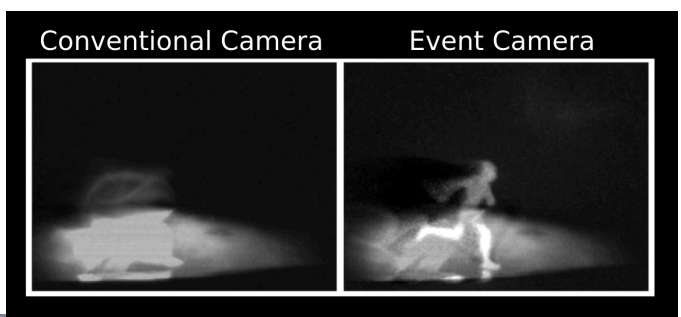
\includegraphics[scale=0.7]{img/event_cameras.png}
    \caption{Difference between standard and event cameras}
\end{figure}

%---------------------------------------------------------
\subsection{Ranging sensors}
They appears as an extension of proximity sensors, since they provide the \textit{distance to objects}. The output of such cameras is an  array of distances (\textit{ranges}) along directions of measurements, or the projection of such distances on the coordinate system of the sensor (\textit{depth}).\\
A 2D array of range is called a \textit{range map}, on the other hand a 2D array of depth is  called a \textit{depth map}. Combing both maps a \textit{point cloud} can be generated. 

\subsubsection{Sonars}
They use \textit{sound waves} to \textbf{detect objects} and \textbf{measure distances} can be either passive or active. The latter ones are very often used in mobile robots coupled with \textit{ultrasonic waves}. A mobile robot not rarely mounts an array of SONAR sensor in order to cover an angular sector of interest. Also in this  case  both piezoelectric and capacitive technologies can be exploited.


\subsubsection{LiDARs (Light Detection and Ranging)}
Such sensors use \textit{infrared lasers} together with reflective properties of the environment in order to measure distances. The generated and received waves can be used in different ways to measure distances.
\begin{enumerate}
    \itemsep-0.3em
    \item \textit{Continuous wave} (also known as phase shift based) exploit the difference in phase between the generated and backscattered wave.
    \item \textit{Pulse Based (PB)} they measure directly the time of flight of a pulse of light, to be interpreted as \textit{round-trip time}.
 \end{enumerate}
 Improved versions of such vanilla version can correct some non-idealities due to light deflections. They can cover higher ranges wrt to sonars and the accuracy is improved. However, they are very sensitive to environmental factors, finally their cost is much higher.

\subsubsection{RADARs (Radio Detection and Ranging)}
They use radiowaves (3mm-30cm), are less accurate with respect to LIDAr, but they can use the \textit{Doppler Effect} to measure distances. They cover a range of 200m in detecting position, relative speed and direction of motion. Briefly speaking, they emit a signal called a \textit{chirp}, whose frequency varies linearly over time. The difference between the frequencies of the emitted and received signal  varies according to the distance of the object to detect.

\subsubsection{ToF cameras}
\textbf{Time of Flight (ToF) cameras} represent the meeting point between LIDARs sensors and digital cameras. Here an infrared wave is emitted and its reflected wave is detected by a 2D imaging sensor. 


\subsubsection{Stereo Cameras}
They are based on the concept of disparity, here triangulation is used in order to reconstruct depths. Such cameras can also be passive: here there are two ordinary cameras, the accuracy in this case is lower, moreover untextured homogeneous areas are hard to be measured.

\begin{figure}[h]
    \centering
    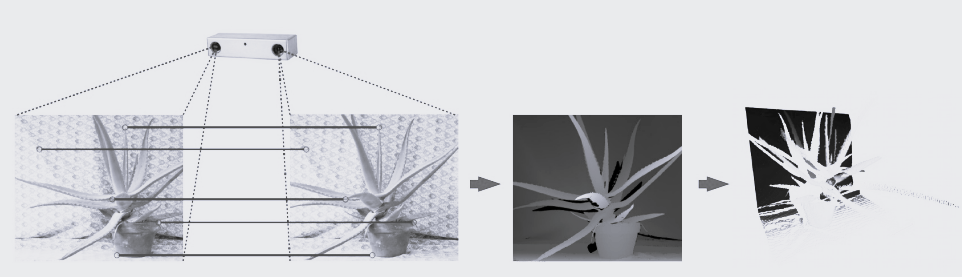
\includegraphics[scale=0.6]{img/stereo_camers.png}
    \caption{Stereo cameras}
\end{figure}

\subsubsection{RGB-D Cameras}
They are particular color cameras which also provide the depth estimates. Even in this case they can be both active or passive. Active cameras use a \textbf{pattern projector}, which creates a saliency map also for homogeneous surfaces.

\begin{figure}
    \centering
    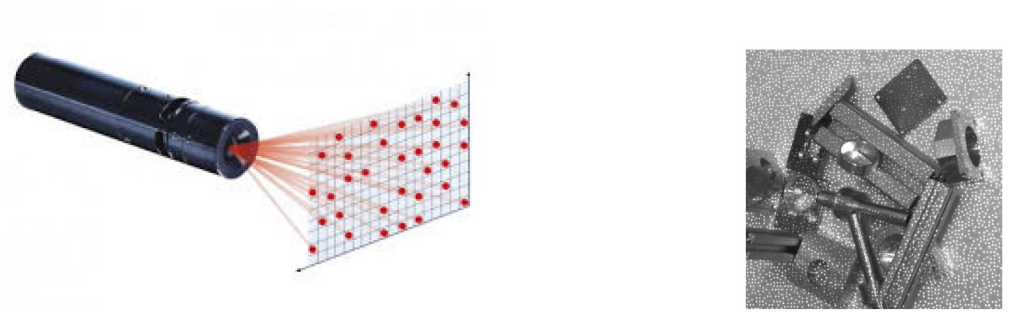
\includegraphics[scale=0.7]{img/pattern_projector.png}
    \caption{Pattern projector}
\end{figure}

\subsubsection{Structured Light Cameras}
They use the same principles of stereo cameras with the only difference that they use instead of two cameras, a single camera and a pattern projector which plays the role of a \textit{virtual camera}. Briefly speaking, their working principle can be summarized as follows: 
\begin{itemize}
    \itemsep-0.3em
    \item \textsf{Projection}  A light source (often a laser or LED) projects a structured pattern onto the object.
    \item \textsf{Capture} A camera records how the pattern distorts.
    \item \textsf{Processing} The system analyzes pattern distortions to calculate depth using triangulation.
\end{itemize}


